\subsection{PSoC}

På figur \ref{fig:ibd_psoc} ses de interne signaler for blokken PSoC.

\begin{figure}[h]
\centering
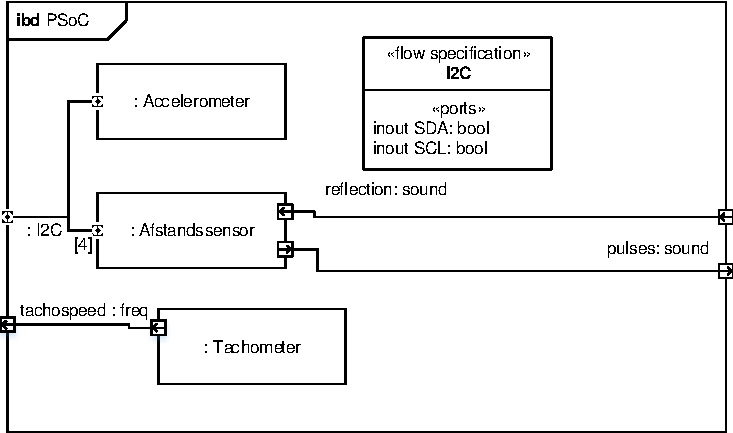
\includegraphics[scale=1]{../fig/diagrammer/bil/ibd_PSoC.pdf}
\caption{IBD for blokken PSoC}
\label{fig:ibd_psoc}
\end{figure}

\subsubsection{Signalbeskrivelse for PSoC}

\begin{table}[h]
	\centering
	\begin{tabularx}{\textwidth}{|l|Z|Z|Z|} \hline
	\textbf{Signal (navn: type)} & \textbf{Funktion} & \textbf{Tolerancer} & \textbf{Kommentarer} \\ \hline
Inout SDA: bool
	& \IIC dataline til sensorer herunder accelerometer og afstandssensorer. 
	& 0-5V $\pm$ 0.5V
 	& Logisk signal: \newline
		Lav = 0V $\pm$ 0.5V \newline
		Høj = 5V $\pm$ 0.5V
	\\ \hline

Inout SCL: bool
	& \IIC clockline  til sensorer herunder accelerometer og afstandssensorer. 
	& 0-5V $\pm$ 0.5V
 	& Logisk signal: \newline
		Lav = 0V $\pm$ 0.5V \newline
		Høj = 5V $\pm$ 0.5V
	\\ \hline

Pulses: sound
	& lydbølger afsendt af sensor. 
	& Ultralydsfrekvens på 42kHz
 	& ~
	\\ \hline
	
reflections: sound
	& Refleksionsbølge fra forhindring. 
	& delay'ed Ultralydsfrekvens på 42kHz
 	& ~
	\\ \hline
	
tachoSpeed: freq
	& Digitalt signal med varierende frekvens afhængig af baghjulenes omdrejningshastighed.
	& ~
	& Vejledende: \newline
		64Hz = 10Km/t \newline
		Logisk signal: \newline
		Lav = 0V +/- 0.2V \newline
		Høj = 5V +/- 0.2V	\\ \hline
	\end{tabularx}
\end{table}